\documentclass[aspectratio=169,10pt]{beamer}
\usetheme{default}
\usecolortheme{default}
\setbeamertemplate{navigation symbols}{}
\setbeamertemplate{footline}[frame number]
\setbeamercolor{frametitle}{fg=black}
\setbeamerfont{frametitle}{series=\bfseries,size=\large}
\usepackage{booktabs}
\usepackage{multirow}
\usepackage{tikz}
\usetikzlibrary{arrows.meta,positioning,fit}
\definecolor{colCo}{HTML}{DCE8F5}
\definecolor{colBG}{HTML}{F6C89F}
\definecolor{colBa}{HTML}{BFE3C8}
\definecolor{colRo}{HTML}{E2D5EE}
\definecolor{acc}{HTML}{3b6fb6}
\setbeamercolor{structure}{fg=acc}
\graphicspath{{figures/}{../figures/}}
\makeatletter
\def\input@path{{figures/}{../figures/}}
\makeatother

\title{Dual-View Address Mapping for NPU--PIM Memory}
\subtitle{Reproducing the PFM address-mapping optimizer on Ramulator 2.0}
\author{Group 13\\[2mm]
{\footnotesize\begin{tabular}{lll}
Yash Gupta & 264101064 & \texttt{yash.g@iitg.ac.in} \\
Nikunj Ladumor & 264101032 & \texttt{nikunj.ladumor@iitg.ac.in} \\
Vamshi Kumar Kanduri & 264101061 & \texttt{vamshi.kanduri@iitg.ac.in} \\
Priyanshu Ganjeer & 264101035 & \texttt{priyanshu.ganje@iitg.ac.in}
\end{tabular}}\\[2mm]
{\small Department of Computer Science and Engineering, IIT Guwahati}}
\date{}
\hypersetup{pdfauthor={Group 13}, pdftitle={Dual-View Address Mapping for NPU-PIM Memory}}

\begin{document}

\begin{frame}
\titlepage
\centering\small Paper: S.~Zhao et al., ``Rethinking Unified Memory for NPU-PIM Systems: Dual-View Memory for Dynamic Inference of LLM'', arXiv:2608.06989
\end{frame}

\begin{frame}{The problem: one matrix, two devices, two wishes}
\begin{columns}[T]
\column{0.48\textwidth}
\textbf{NPU} (prefill, large GEMM)
\begin{itemize}
\item reads weights as one long sequential stream
\item wants consecutive addresses on \emph{different} banks / bank groups / channels
\item so the data bus never waits
\end{itemize}
\column{0.48\textwidth}
\textbf{PIM} (decode, GEMV)
\begin{itemize}
\item one small compute unit next to each bank
\item one command drives \emph{all banks at once}
\item wants each unit's weight column \emph{inside its own bank}
\end{itemize}
\end{columns}
\vspace{6mm}
\begin{block}{}
A shared memory stores each weight matrix once, so it has \textbf{one} physical layout.\\
PFM: pick one layout per 2\,MB page that is good for both, with an integer program.
\end{block}
\end{frame}

\begin{frame}{Assignment scope}
\begin{itemize}
\item Implement the address-mapping optimizer (Python + PuLP)
\item In Ramulator 2.0, add a mapping choice per memory region
\item Compare three layouts: \textbf{NPU-friendly}, \textbf{PIM-friendly}, \textbf{jointly optimized}
\item Report bandwidth utilization for NPU sequential reads and PIM matrix-vector access
\item Use the LLaMA3-8B weight shapes
\end{itemize}
\vspace{3mm}
\begin{center}
\small
\begin{tabular}{lrr}
\toprule
Matrix ($d_{in}\times d_{out}$) & Shape & 2\,MB pages \\
\midrule
q\_proj, o\_proj & 4096$\times$4096 & 16 each \\
k\_proj, v\_proj & 4096$\times$1024 & 4 each \\
gate\_proj, up\_proj & 4096$\times$14336 & 56 each \\
down\_proj & 14336$\times$4096 & 56 \\
\bottomrule
\end{tabular}
\end{center}
Out of scope: GPU kernels, hardware synthesis, larger models.
\end{frame}

\begin{frame}{DRAM background in two facts}
\begin{enumerate}
\item \textbf{Row buffer.} Reading the open row is fast. Another row costs precharge + activate $= 16+16$ cycles (DDR4-2400).
\item \textbf{Bank groups.} Two reads to the \emph{same} bank group: 6 cycles apart ($t_{CCD\_L}$). To \emph{different} groups: 4 cycles ($t_{CCD\_S}$).\\
A 64\,B burst uses the bus for 4 cycles $\Rightarrow$ staying in one group caps bandwidth at $4/6 = 66.7\%$.
\end{enumerate}
\vspace{4mm}
\begin{block}{Address mapping}
Which address bit picks the column, bank group, bank or row.\\
A 2\,MB page has $2^{21}/64 = 32768$ lines $\Rightarrow$ \textbf{15 free bits} to assign.\\
DDR4 x8: 7 column, 2 bank-group, 2 bank, 4 row bits.
\end{block}
\small On DDR4, bank-group bits play the role of the paper's HBM channel bits.
\end{frame}

\begin{frame}{The PIM ``unit window''}
\begin{itemize}
\item Weights stored column by column: one column = $d_{in}\times 2$\,B $= 2^{p_n}$ lines
\item[] $p_n = 7$ for $d_{in}=4096$, \quad $p_n = 9$ for $d_{in}=14336$ (padded to 16384)
\item Line index $= c \cdot 2^{p_n} + t$ \quad (column $c$, offset $t$)
\item 16 PIM units (one per bank); unit $u$ gets columns $c = 16g + u$
\item[$\Rightarrow$] the unit number sits in bits $p_n \ldots p_n{+}3$: the \textbf{unit window}
\end{itemize}
\vspace{4mm}
\begin{block}{Rule}
PIM is fast only if every bit in the unit window is a bank or bank-group bit
(then every unit has its own bank).
\end{block}
\end{frame}

\begin{frame}[fragile]{What we built}
\centering
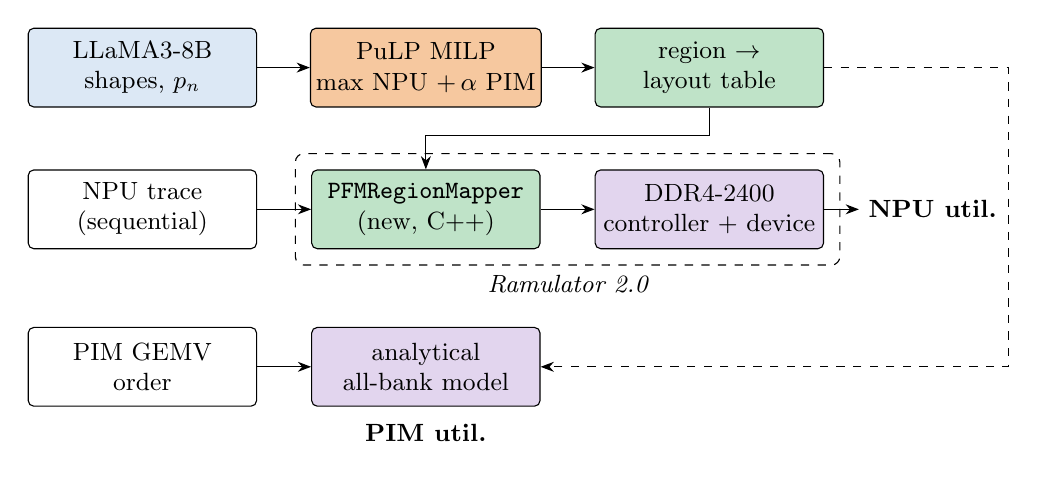
\begin{tikzpicture}[font=\small,
  box/.style={draw, rounded corners=2pt, align=center, minimum height=10mm, minimum width=29mm, inner sep=2pt, fill=#1},
  box/.default=white, >=Stealth]
\node[box=colCo] (shape) at (0,0) {LLaMA3-8B\\shapes, $p_n$};
\node[box=colBG] (milp) at (3.6,0) {PuLP MILP\\max NPU $+\,\alpha$ PIM};
\node[box=colBa] (tab) at (7.2,0) {region $\rightarrow$\\layout table};
\node[box] (npu) at (0,-1.8) {NPU trace\\(sequential)};
\node[box=colBa] (map) at (3.6,-1.8) {\texttt{PFMRegionMapper}\\(new, C++)};
\node[box=colRo] (ctl) at (7.2,-1.8) {DDR4-2400\\controller + device};
\node[box] (pim) at (0,-3.8) {PIM GEMV\\order};
\node[box=colRo] (model) at (3.6,-3.8) {analytical\\all-bank model};
\node[draw, dashed, rounded corners=3pt, fit=(map)(ctl), inner sep=2mm,
      label={[font=\small\itshape]below:Ramulator 2.0}] {};
\draw[->] (shape) -- (milp); \draw[->] (milp) -- (tab);
\draw[->] (tab.south) -- ++(0,-0.35) -| (map.north);
\draw[->] (npu) -- (map); \draw[->] (map) -- (ctl); \draw[->] (pim) -- (model);
\node[anchor=west] (o1) at (9.1,-1.8) {\textbf{NPU util.}}; \draw[->] (ctl) -- (o1);
\draw[->, dashed] (tab.east) -- (11.0,0) |- (model.east);
\node[below=1mm of model] {\textbf{PIM util.}};
\end{tikzpicture}
\vspace{3mm}
\begin{itemize}\small
\item Metric: utilization $= 4 \times \text{reads} / \text{DRAM cycles}$, checked against Ramulator's own throughput counter
\item Every run checks: layout is one-to-one, no duplicate addresses, all reads reach DRAM
\end{itemize}
\end{frame}

\begin{frame}[fragile]{New in Ramulator 2.0: a mapping choice per memory region}
\begin{columns}[T]
\column{0.5\textwidth}
\small
\texttt{PFMRegionMapper}: one new C++ address mapper (about 150 lines)
\begin{itemize}
\item splits memory into 2\,MB regions
\item holds a list of layouts and a table: region $\rightarrow$ layout
\item maps every request with its region's layout
\item checks each layout matches the DRAM's bit counts
\end{itemize}
\vspace{1mm}
\scriptsize
\begin{verbatim}
addr_mapper = PFMRegionMapper(
  layouts=["bg1 col6 bank1 col1 bank1 bg1 row4",
           "bg1 col6 row2 col1 bank2 bg1 row2"],
  region_layout=[0,0,0,0,0,0,1,1])
\end{verbatim}
\column{0.48\textwidth}
\small
\textbf{Check 1:} all 20 layouts give \emph{identical} cycle counts to an independent Python implementation.\\[2mm]
\textbf{Check 2:} one run over 8 regions (6 $\times$ $d_{in}$=4096, 2 $\times$ down\_proj):\\[1mm]
\begin{tabular}{lr}
\toprule
Plan & NPU \% \\
\midrule
NPU-friendly everywhere & 95.05 \\
PIM-friendly everywhere & 65.81 \\
PFM $\alpha$=0.25, 2 layouts & 93.70 \\
PFM $\alpha$=2, 2 layouts & 64.70 \\
\bottomrule
\end{tabular}\\[1mm]
Switching layouts between regions costs almost nothing.
\end{columns}
\end{frame}

\begin{frame}{First measurement: bank-group bits decide NPU bandwidth}
\centering
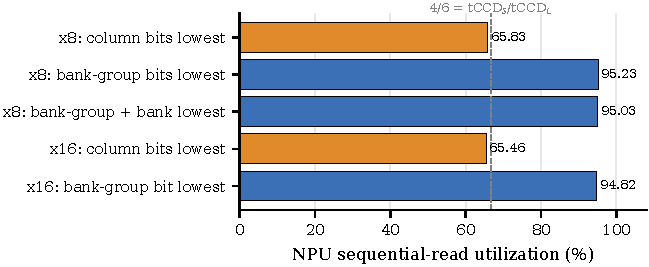
\includegraphics[width=0.72\textwidth]{bg_effect.pdf}
\begin{itemize}\small
\item Column bits lowest: every read stays in one bank group $\Rightarrow$ 66\% (the $4/6$ limit)
\item One bank-group bit at the bottom $\Rightarrow$ 95\%. Row hits are $>$99\% in both cases.
\end{itemize}
\end{frame}

\begin{frame}{The optimizer (MILP)}
Binary $x_{l,j} = 1$ if bit $j$ selects level $l \in \{\text{Co}, \text{BG}, \text{Ba}, \text{Ro}\}$
\begin{itemize}
\item Each bit gets exactly one level: $\sum_l x_{l,j} = 1$
\item Each level gets exactly its bit count: $\sum_j x_{l,j} = B_l$
\end{itemize}
\vspace{2mm}
\textbf{NPU score}: $\tfrac{2}{3} + \tfrac{1}{3}\,[\text{BG bit at position 0}] - \lambda\cdot[\text{row bits below column bits}]$\\[2mm]
\textbf{PIM score}: $2^{-(\text{missing bank bits in window})}\cdot 0.5^{(\text{row bits in window})}$\\[2mm]
\textbf{Objective}: maximize NPU $+\ \alpha \cdot$ PIM \quad (solved with CBC)
\vspace{3mm}
\begin{block}{Checks}
MILP value = exact score of its own answer; it ties or beats 20,000--100,000 random layouts every time; re-running reproduces every stored layout.
\end{block}
\end{frame}

\begin{frame}{PIM model}
Stock Ramulator 2.0 has no PIM commands, so PIM utilization is computed from Ramulator's DDR4-2400 timings:
\begin{itemize}
\item one step = all 16 units read offset $t$ of their current column
\item cost per unit: 6 cycles, $+16$ if the bank is closed, $+32$ if the row changes
\item units in the same bank add up; the step takes as long as the slowest bank
\item utilization = ideal time / modeled time
\end{itemize}
\vspace{4mm}
\small We also replayed the same order as normal reads in Ramulator. The scheduler reorders those reads and hides bank conflicts, so this proxy was too lenient (about 95\% for almost every layout). It is kept only as a cross-check.
\end{frame}

\begin{frame}{Baseline results}
\centering
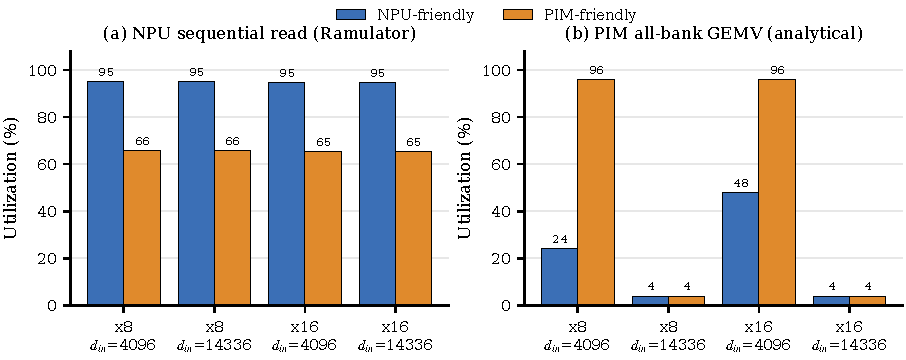
\includegraphics[width=\textwidth]{baseline.pdf}
\begin{itemize}\small
\item Each fixed layout is good for one device only
\item For $d_{in}=14336$ (down\_proj) the unit window holds row bits: \textbf{4\% PIM} for both
\end{itemize}
\end{frame}

\begin{frame}{Layouts found by the optimizer (DDR4 x8)}
\centering
\resizebox{0.78\textwidth}{!}{\input{layouts_tikz.tex}}\\[1mm]
\small Red box = PIM unit window. Co column, BG bank group, Ba bank, Ro row.
\end{frame}

\begin{frame}{Contribution results}
\centering
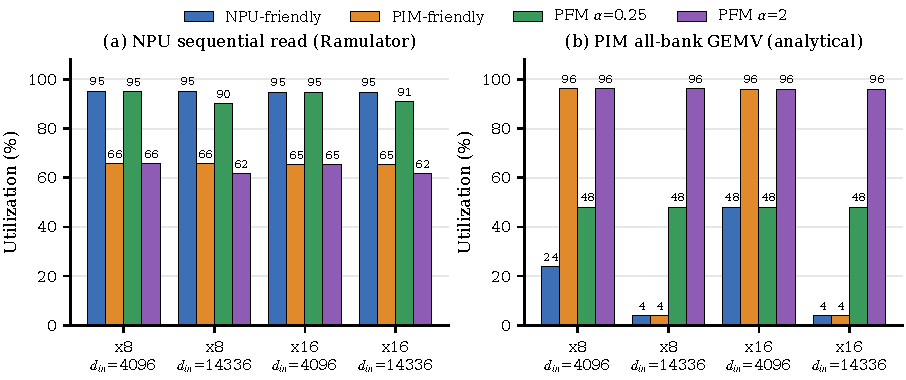
\includegraphics[width=\textwidth]{contribution.pdf}
\begin{itemize}\small
\item PFM $\alpha=0.25$: NPU stays at 90--95\%, PIM goes $24\rightarrow48\%$ and $4\rightarrow48\%$
\item PFM $\alpha=2$: best PIM (96\%) everywhere, including down\_proj\\(note: the fixed baselines were designed for $d_{in}$=4096; part of the down\_proj gain is adapting to its shape)
\end{itemize}
\end{frame}

\begin{frame}{Whole LLaMA3-8B decoder layer}
\centering
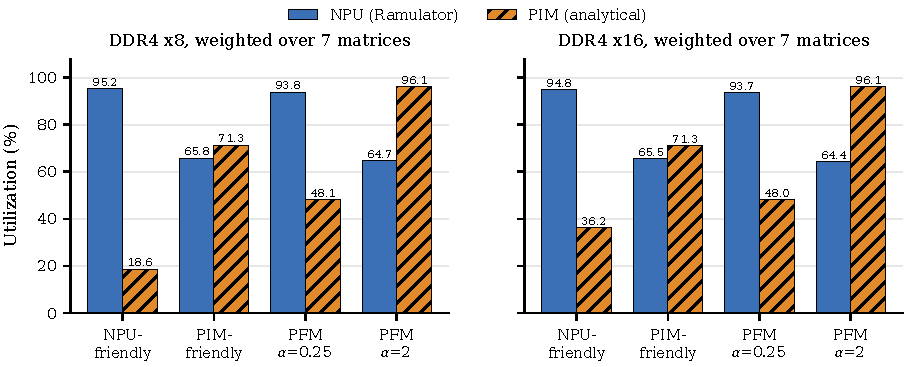
\includegraphics[width=0.95\textwidth]{llama_weighted.pdf}
\begin{itemize}\small
\item $\alpha=0.25$ vs NPU-friendly: $-1.4$ NPU points, $+29.4$ PIM points (18.6\% $\rightarrow$ 48.1\%)
\item $\alpha=2$ vs PIM-friendly: $+24.8$ PIM points (71.3\% $\rightarrow$ 96.1\%) for $-1.1$ NPU points
\end{itemize}
\end{frame}

\begin{frame}{Why no layout wins both on DDR4, and what $\alpha$ does}
\begin{columns}[T]
\column{0.5\textwidth}
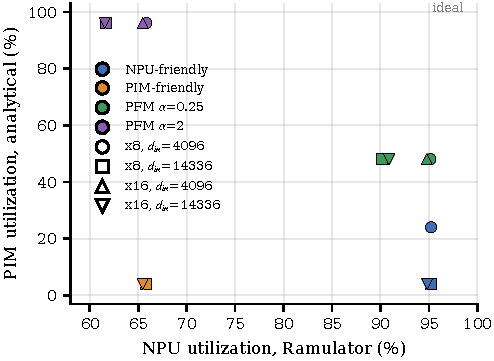
\includegraphics[width=\textwidth]{tradeoff.pdf}
\column{0.48\textwidth}
\small
\textbf{Bit budget.} x8 has only 4 bank-level bits.
\begin{itemize}
\item NPU needs 1 of them at bit 0
\item PIM needs all 4 in the unit window
\item[$\Rightarrow$] at most 3 in the window $\Rightarrow$ PIM $\le 50\%$ when NPU is at full speed
\end{itemize}
The paper's HBM has extra channel bits for the NPU, so it avoids this.
\vspace{2mm}

\textbf{$\alpha$} picks the point on the trade-off: switch at $\alpha \approx 2/3$.\\
Low $\alpha$: prefill-heavy serving. High $\alpha$: decode-heavy.
\end{columns}
\end{frame}

\begin{frame}{How good are the models?}
\begin{columns}[T]
\column{0.5\textwidth}
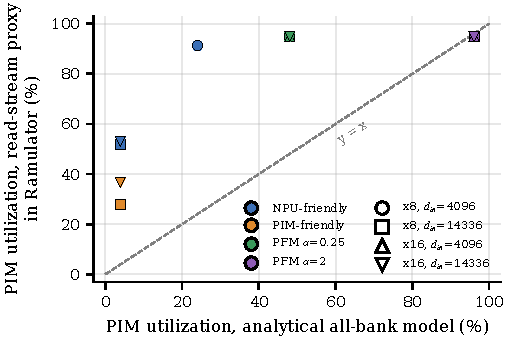
\includegraphics[width=\textwidth]{proxy_vs_model.pdf}
\column{0.48\textwidth}
\small
\begin{itemize}
\item \textbf{NPU score vs Ramulator}: 1.00 $\leftrightarrow$ 95.2\%, 0.67 $\leftrightarrow$ 65.8\%, 0.98 $\leftrightarrow$ 90.2\% (3 points optimistic)
\item \textbf{PIM}: the read proxy says $\approx$95\% for most layouts because the scheduler reorders reads; a lock-step PIM command cannot
\item So PIM numbers come from the analytical model
\end{itemize}
\end{columns}
\end{frame}

\begin{frame}{Limitations}
\begin{enumerate}
\item PIM utilization is analytical, not cycle-simulated; it shares its main assumption with the optimizer
\item Single-channel DDR4, not multi-channel HBM2e-PIM; the paper's numbers are not reproduced
\item The fixed baselines are designed for $d_{in}=4096$, so they are weak on down\_proj
\item Static layouts per tensor class; no runtime scheduling or hardware validation
\end{enumerate}
\end{frame}

\begin{frame}{Conclusion}
\begin{itemize}
\item Verified PuLP MILP that maps 15 address bits per 2\,MB page
\item New Ramulator mapper \texttt{PFMRegionMapper}: a layout per 2\,MB region, checked cycle-for-cycle
\item Joint layouts raise PIM utilization at nearly the same NPU utilization:\\
\quad 18.6\% $\rightarrow$ 48.1\% PIM at 93.8\% NPU over a decoder layer
\item down\_proj: 4\% $\rightarrow$ 48--96\% PIM
\item On single-channel DDR4 the bit budget forces a trade-off, and $\alpha$ selects it
\end{itemize}
\vspace{4mm}
\textbf{Next:} multiple channels, PIM commands inside Ramulator for a cycle-level PIM model.\\[4mm]
\small Source code: \url{https://github.com/groupiitg/PFM}\par
\vspace{4mm}
{\centering \Large Thank you. Questions?\par}
\end{frame}

\end{document}
